\documentclass{article}
\usepackage{tabularx}
\usepackage{graphicx}
\usepackage{dirtytalk}
\usepackage{pgfplotstable} 
\usepackage{pgfplots}
\usepackage{datatool}
\usepackage{siunitx}
\usepackage[hyphens]{url}
\usepackage{hyperref}
\usepackage{graphicx}
\usepackage{microtype}
\usepackage{float}
\usepackage[style=ieee]{biblatex}
\usepackage{listings}
\usepackage{xcolor}
\usepackage[normalem]{ulem}
\usepackage{dirtytalk}

\definecolor{mygreen}{rgb}{0,0.6,0}
\definecolor{mygray}{rgb}{0.5,0.5,0.5}
\definecolor{mymauve}{rgb}{0.58,0,0.82}

\lstset{
    language=Java,                % Set language to Java
    basicstyle=\ttfamily\footnotesize, % Set font style and size
    keywordstyle=\color{blue},    % Set color for keywords
    stringstyle=\color{mymauve},  % Set color for strings
    commentstyle=\color{mygreen}, % Set color for comments
    numbers=left,                 % Line numbers on the left
    numberstyle=\tiny\color{mygray}, % Style for line numbers
    stepnumber=1,                 % Line number step size
    numbersep=10pt,               % Line number separation
    backgroundcolor=\color{white},% Background color
    showspaces=false,             % Do not show spaces
    showstringspaces=false,       % Do not underline spaces in strings
    showtabs=false,               % Do not show tabs
    frame=single,                 % Draw a frame around the code
    tabsize=4,                    % Set tab size
    captionpos=b,                 % Caption position (bottom)
    breaklines=true,              % Allow line breaking
    breakatwhitespace=false,      % Line breaks only at whitespace
    title=\lstname                % Show the filename of the code
}

\lstdefinestyle{bash}{
    language=bash,                % Set language to Bash
    basicstyle=\ttfamily\footnotesize, % Set font style and size
    keywordstyle=\color{blue},    % Set color for keywords
    stringstyle=\color{mymauve},  % Set color for strings
    commentstyle=\color{mygreen}, % Set color for comments
    numbers=left,                 % Line numbers on the left
    numberstyle=\tiny\color{mygray}, % Style for line numbers
    stepnumber=1,                 % Line number step size
    numbersep=10pt,               % Line number separation
    backgroundcolor=\color{white},% Background color
    showspaces=false,             % Do not show spaces
    showstringspaces=false,       % Do not underline spaces in strings
    showtabs=false,               % Do not show tabs
    frame=single,                 % Draw a frame around the code
    tabsize=4,                    % Set tab size
    captionpos=b,                 % Caption position (bottom)
    breaklines=true,              % Allow line breaking
    breakatwhitespace=false,      % Line breaks only at whitespace
    title=\lstname                % Show the filename of the code
}

\addbibresource{main.bib}

\hypersetup{
    colorlinks=true,
    linkcolor=blue,
    filecolor=blue,      
    urlcolor=blue,
    citecolor=blue,
}

\pgfplotsset{compat=1.18}

\title{\textbf{Lab 3 - Linearizability of Lock-free Skiplists\\Parallel and Distributed Computing\\DD2443 - Pardis24}}
\author{Names:\\Casper Kristiansson\\Nicole Wijkman\\\\Group 14}
\date{\today}

\begin{document}

\setlength\parindent{0pt}
\setlength{\parskip}{\bigskipamount}

\maketitle

\newpage
\section{Measuring Execution Time}

\subsection{Measurement program \& Dardel experiments}

\subsubsection{Explanation}
The execution time of the \texttt{LockFreeSkipList} was measured using a custom program with thread counts of 1, 2, 4, and 8. The operations were split into two mixtures: 10\% add, 10\% remove, and 80\% contains (1:1:8), and 50\% add and 50\% remove (1:1:0). The values were sampled from both normal and uniform distributions. Each thread executed 100,000 operations with 5 warmup rounds and 10 measurement rounds for final statistics.

The program was also run on Dardel (PDC) using thread counts up to 96. The same mixtures and distributions were applied, simulating larger workloads to observe scaling performance under higher contention.

\subsubsection{Results and Plots}

The following figures show the performance of the LockFreeSkipList with both normal and uniform distributions, across a range of thread counts.

\begin{figure}[H]
    \centering
    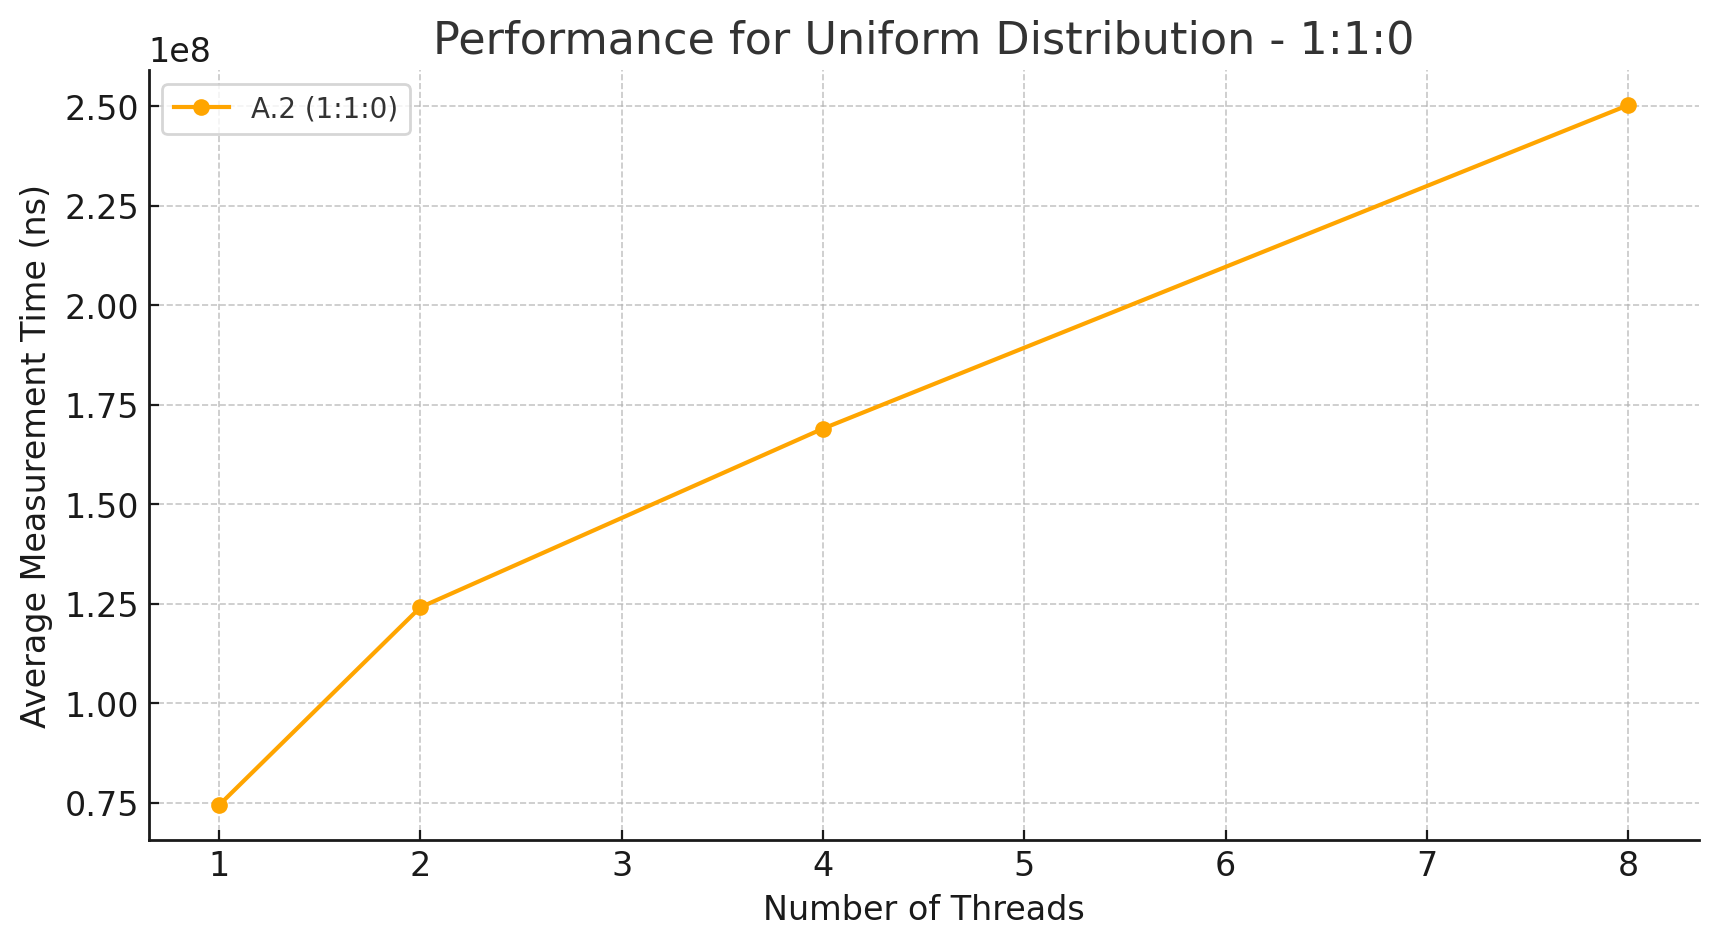
\includegraphics[width=\textwidth]{LaTex/images/Lab 3 1.2.1.png}
    \caption{Performance for Uniform Distribution - 1:1:0}
    \label{fig:enter-label}
\end{figure}

\begin{figure}[H]
    \centering
    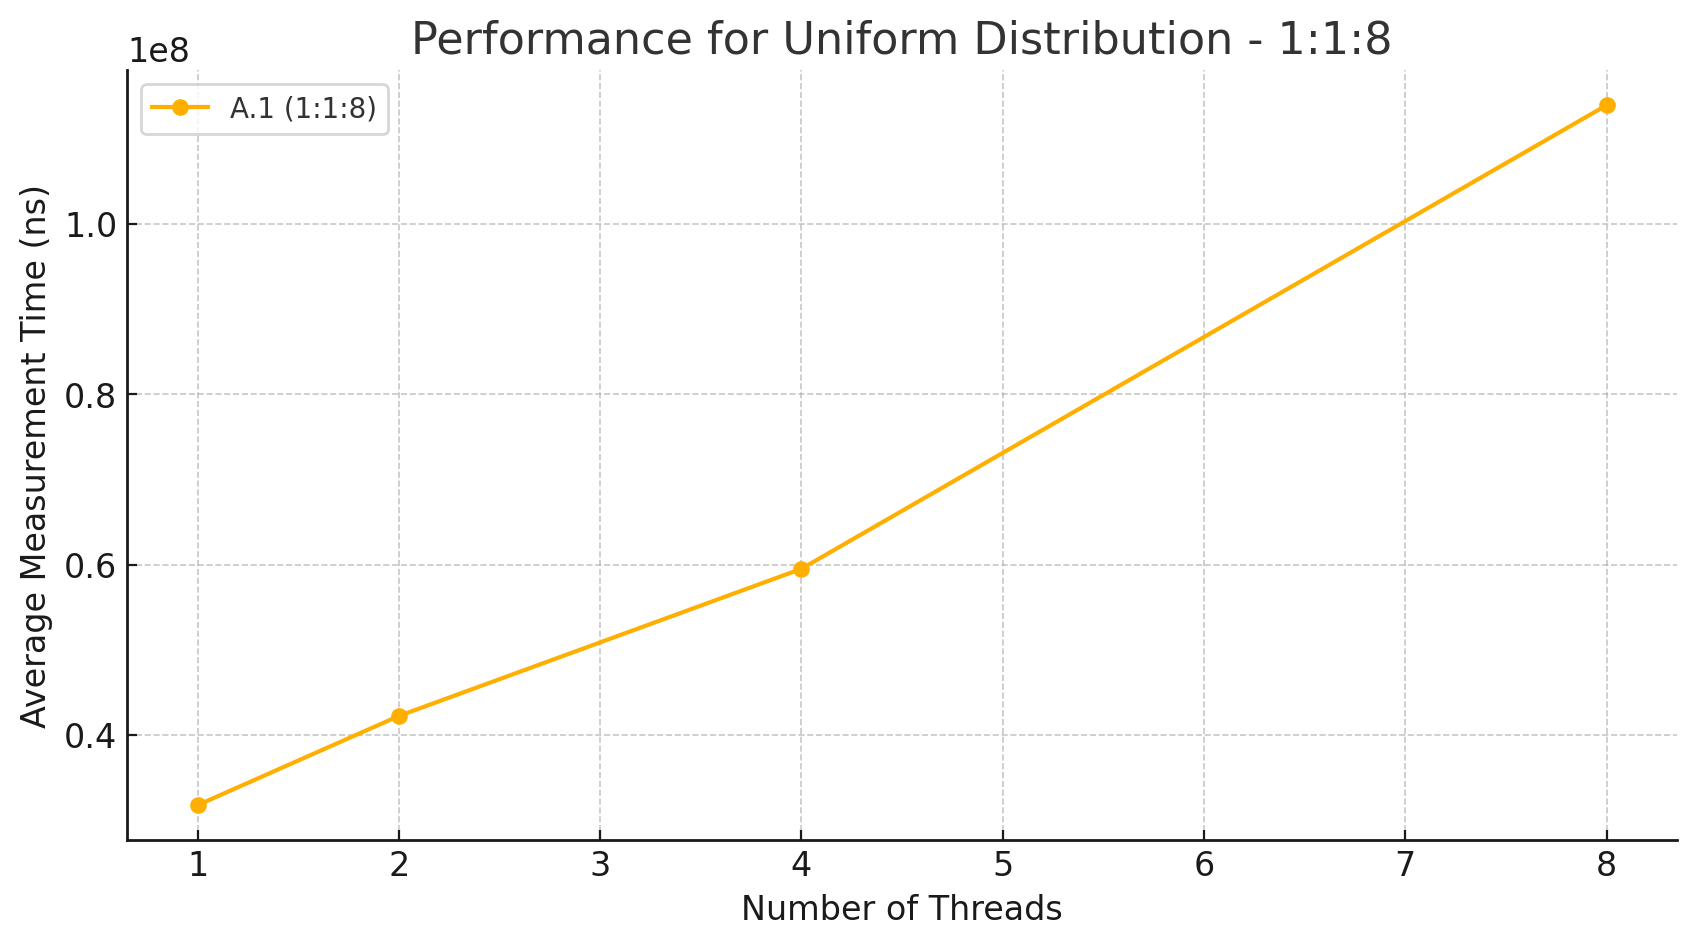
\includegraphics[width=\textwidth]{LaTex/images/Lab 3 1.2.2.png}
    \caption{Performance for Uniform Distribution - 1:1:8}
    \label{fig:enter-label}
\end{figure}

\begin{figure}[H]
    \centering
    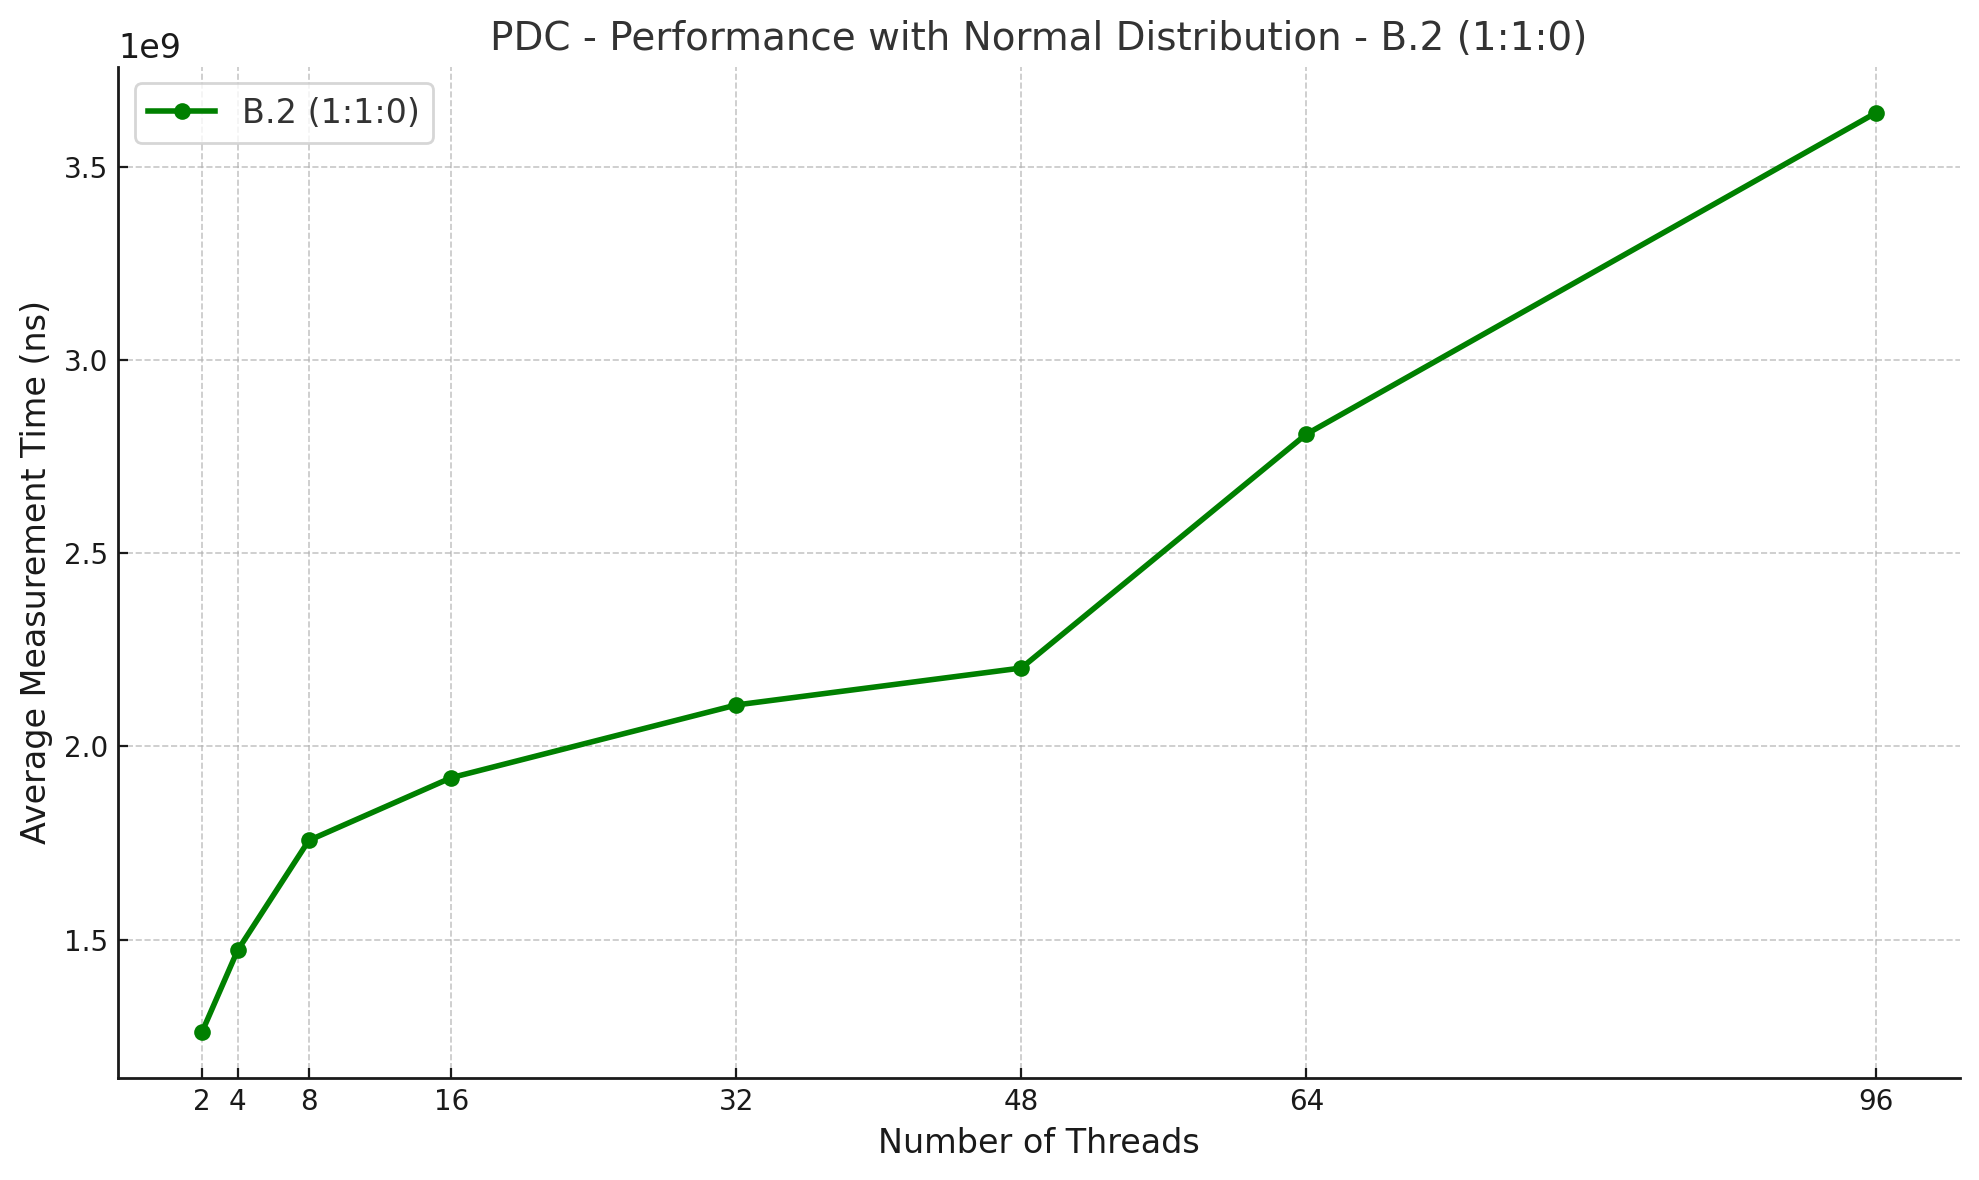
\includegraphics[width=\textwidth]{LaTex/images/Lab 3 1.2.3.png}
    \caption{PDC - Performance for Normal Distribution - 1:1:0}
    \label{fig:enter-label}
\end{figure}

\begin{figure}[H]
    \centering
    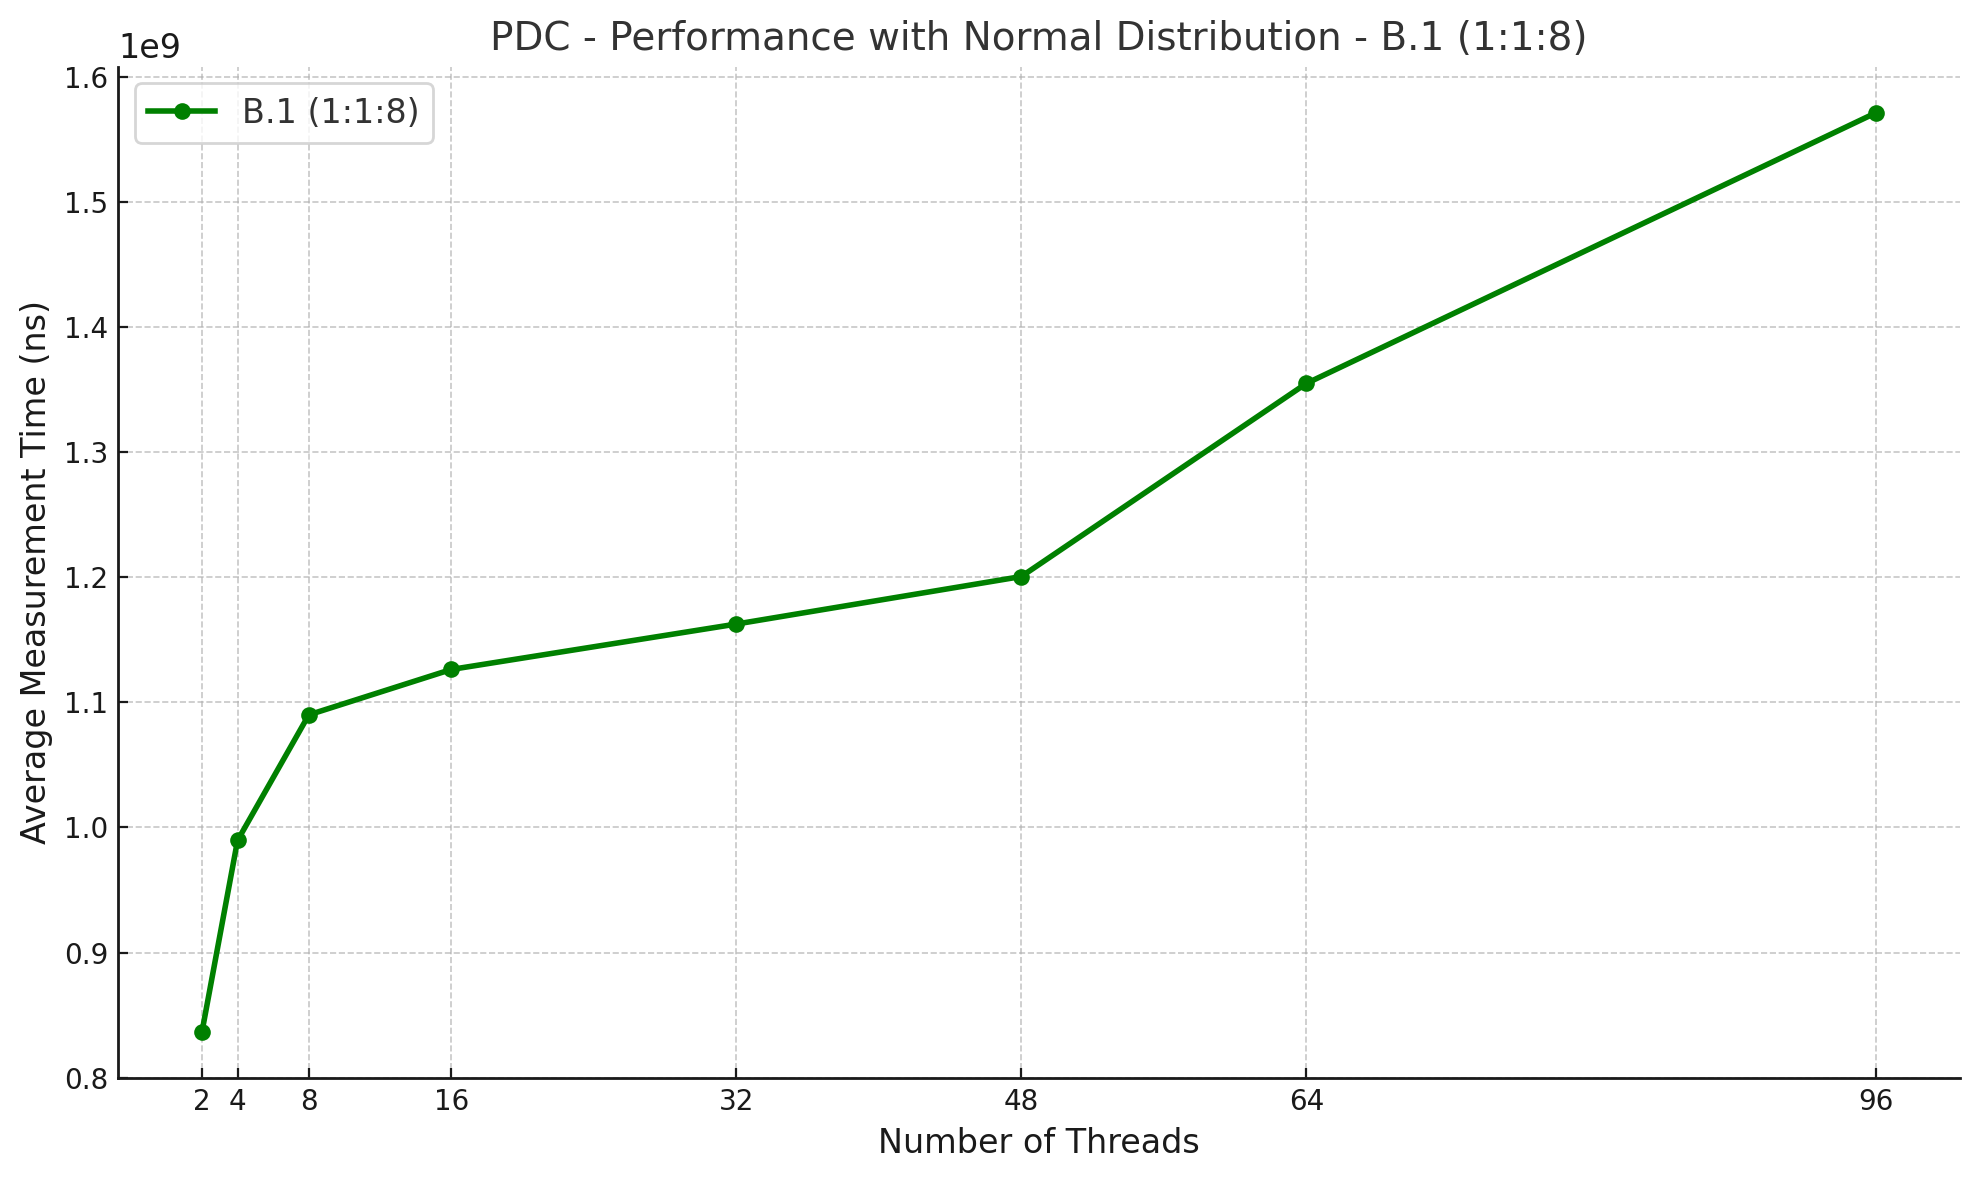
\includegraphics[width=\textwidth]{LaTex/images/Lab 3 1.2.4.png}
    \caption{PDC - Performance for Normal Distribution - 1:1:8}
    \label{fig:enter-label}
\end{figure}

\subsubsection{Discussion}
The results indicate that execution time increases with the number of threads, especially beyond 4 threads. This pattern holds across both the normal and uniform distributions and both operation mixtures. The initial decrease in execution time with up to 4 threads is due to improved parallelism. However, the overhead of managing higher thread counts causes the execution time to rise again with 8 threads.

In the Dardel experiments (Figures 3 and 4), the trends observed in local measurements are confirmed. As the number of threads increases up to 96, the performance degradation becomes more apparent, particularly for the 1:1:0 mixture. The read-heavy mixture (1:1:8) initially scales better, but with high thread counts, contention on shared resources becomes the limiting factor, leading to slower execution times.

The increased execution time with more threads is especially pronounced in the normal distribution cases (Figures 3 and 4). This is likely due to the distribution characteristics, where normal distribution results in a higher concentration of operations around the mean, increasing contention on certain key ranges.


\newpage
\section{Identifying and Validating Linearization Points}

\subsection{Identify Linearization Points}

\subsubsection{Explanation}
The linearization points are the moments when operations appear to take effect atomically, ensuring the correctness of the concurrent data structure.

For the \texttt{add()} method, the linearization point remains when the \texttt{compareAndSet()} succeeds on the bottom-level reference, linking the new node into the list. However, now the exact timestamp for this operation is captured using \texttt{System.nanoTime()} immediately after a successful \texttt{compareAndSet()} to ensure accurate timing. If the node is already present, the linearization point is observed during the \texttt{find()} operation when it determines the node’s presence, and the timestamp is captured accordingly.

In the \texttt{remove()} method, the linearization point occurs when the \texttt{compareAndSet()} marks the bottom-level node for removal. The timestamp is captured after the successful marking operation to accurately represent the time of the linearization point. For unsuccessful removals, the \texttt{find()} operation aids in detecting the correct linearization point by checking if a node has been logically removed (marked) and logging the timestamp for validation purposes.

For the \texttt{contains()} method, the linearization point is identified when it checks the bottom-level list and determines if the target node is unmarked. If the target key is found, the success is marked with a timestamp at that point, and if the key is missing, the failure is timestamped accordingly.

\subsubsection{Discussion}
The linearization points for \texttt{add()}, \texttt{remove()}, and \texttt{contains()} are based on atomic \texttt{compareAndSet()} operations, ensuring consistency across threads. In this implementation, precise timing using \texttt{System.nanoTime()} is captured immediately after critical operations like successful \texttt{compareAndSet()} or after confirming the status through \texttt{find()} checks. This ensures that the linearization points are accurately represented in the logs, maintaining the appearance of atomicity, which is crucial for ensuring correct and efficient concurrent behavior.




\newpage
\subsection{Developing a Validation Method}

\subsubsection{Explanation}
The \texttt{LogEntry} class was designed to capture the linearization points by recording the method name (for example: \texttt{add()}, \texttt{remove()}, or \texttt{contains()}), the arguments (the hash code of the element), the return value (e.g., success or failure), and the exact timestamp using \texttt{System.nanoTime()}. For validation, the \texttt{Log.validate} method replays the log entries on a \texttt{HashSet} and compares the results. If the \texttt{add()} method returns true in the log but the \texttt{HashSet} shows it as false, this counts as a discrepancy. The number of discrepancies indicates the consistency of the log.

\subsubsection{Discussion}
The validation method worked effectively for capturing the linearization points for the \texttt{add()} and \texttt{remove()} operations, resulting in a low discrepancy count. The challenge was ensuring that the \texttt{contains()} method properly captures linearization points, as this operation only checks for the existence of an element and does not modify the skiplist, making it harder to validate with the same accuracy as \texttt{add()} and \texttt{remove()}. However, the overall log validation showed consistent and reliable behavior.

\newpage
\subsection{Locked Time Sampling}

\subsubsection{Explanation}
The locked time sampling method employs a \texttt{ReentrantLock} to synchronize the linearization point and time sampling. The lock ensures that no other threads can interleave, thereby capturing an accurate timestamp. In the \texttt{remove()} method, after a successful \texttt{compareAndSet()}, the timestamp is captured with \texttt{System.nanoTime()}. This ensures atomicity between the linearization point and time sampling. The same pattern is followed in the \texttt{add()} and \texttt{contains()} methods, providing consistency in time capture across all operations.

\subsubsection{Results and Plots}

The following plot shows the performance of the locked time sampling method under different operation mixtures. The x-axis represents the number of threads, and the y-axis represents the average measurement time in nanoseconds.


\begin{figure}[H]
    \centering
    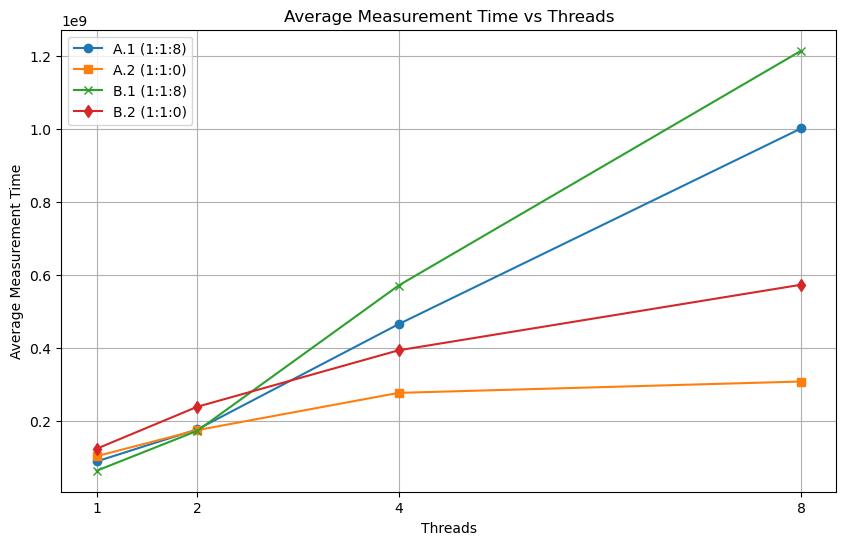
\includegraphics[width=\textwidth]{LaTex/images/Lab 3 2.3.2.1.png}
    \caption{Measurement Time vs Threads}
    \label{fig:fig5}
\end{figure}

\subsubsection{Discussion}
The locked time sampling method provided accurate time measurements across all tested thread counts, but with a slight increase in latency due to the use of locks. As expected, the synchronization overhead led to a gradual rise in measurement time as the number of threads increased, particularly for mixtures involving a higher proportion of write operations.

Figure \ref{fig:fig5} illustrates that execution time scales with the number of threads. In the mixture involving 80\% contains operations (A.1 and B.1), the measurement time grows more significantly, particularly in scenarios with more threads. This indicates that as the number of operations increases, the contention overhead becomes more noticeable due to the locking mechanism.

In comparison to previous methods, the locked time sampling still ensures that both the linearization point and time sampling are closely aligned, providing higher accuracy at the cost of slightly increased overhead. This method remains effective when accurate synchronization is essential, and the trade-off in performance is acceptable.

\newpage
\subsection{Lock-free Time Sampling with Local Log}

\subsubsection{Explanation}
In the lock-free time sampling method with local logs, each thread maintains its own local log, recording operations and time samples without any global lock. This reduces synchronization overhead and allows each thread to operate independently. At the end of the experiment, the local logs from each thread are merged into a global log and sorted by timestamp for validation. While this approach improves performance by avoiding global synchronization, it introduces the possibility of discrepancies due to interleaving between time sampling and the linearization point.

\subsubsection{Results and Plots}

The following plot shows the performance of the lock-free time sampling method with local logs in different operation mixtures. The x-axis represents the number of threads, and the y-axis represents the measurement time in nanoseconds.


\begin{figure}[H]
    \centering
    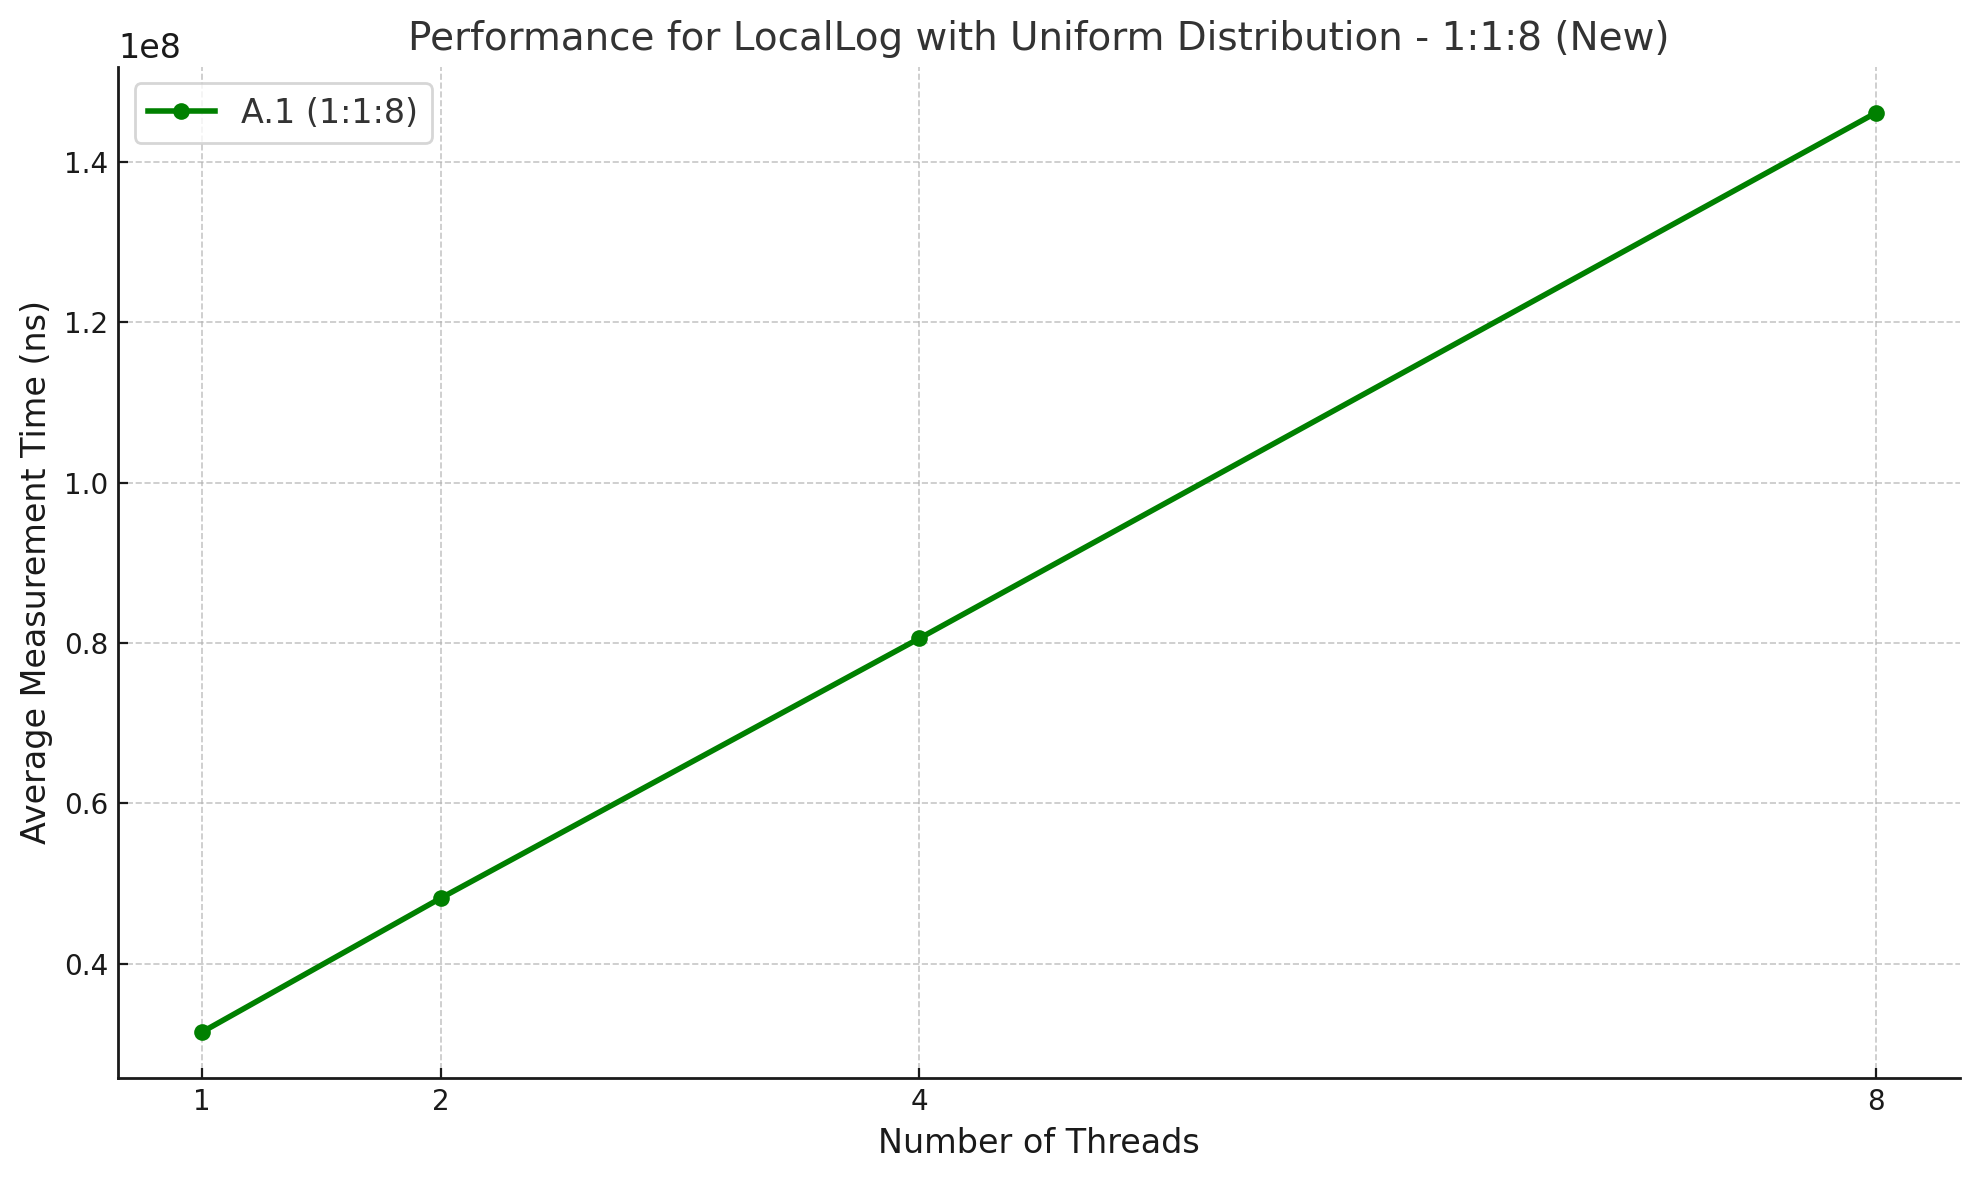
\includegraphics[width=0.9\textwidth]{LaTex/images/Lab 3 2.4.2.1.png}
    \caption{Performance for LocalLog}
    \label{fig:performance_a1}
\end{figure}


On Dardel, we measured both the execution time and the accuracy of the logs, using the same experimental cases from Task 1.2. The following plot show the execution time for the lock-free time sampling method with local logs under normal distribution scenarios.

\begin{figure}[H]
    \centering
    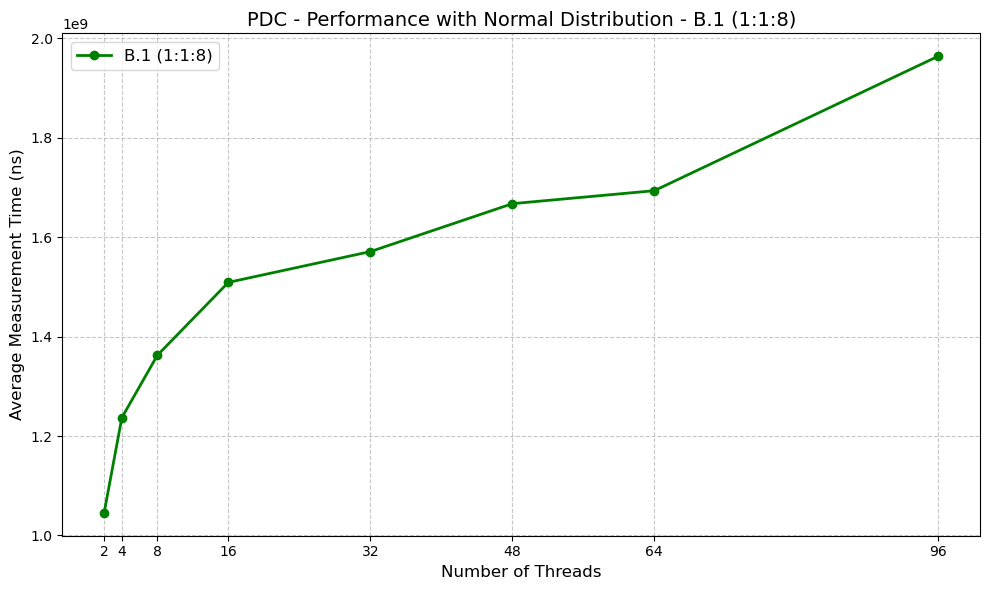
\includegraphics[width=0.9\textwidth]{LaTex/images/Lab 3 2.4.2.3.png}
    \caption{Performance for LocalLog - on Dardel}
    \label{fig:performance_dardel_1}
\end{figure}


\subsubsection{Discussion}
The lock-free local logging approach effectively reduces synchronization overhead by avoiding global locks, thus enhancing performance, especially with lower thread counts. As shown in the figures, the execution time scales predictably with the increase in the number of threads for both uniform and normal distributions. This demonstrates that the method remains efficient as concurrency increases, showing minimal overhead even at higher thread counts.

In scenarios with thread counts of 1, 2, or 4, discrepancies were minimal due to the reduced contention, allowing time sampling to closely align with the linearization points. With thread counts of 8 and higher, minor discrepancies were detected, likely resulting from the higher concurrency leading to slight interleaving between time sampling and the actual linearization point. Despite this, the discrepancy count remained manageable, indicating that the method retains sufficient accuracy for workloads with moderate contention.

The Dardel experiments, which reached up to 48 threads, confirmed the scalability of the lock-free local logging method in environments with high concurrency. The results show that execution time generally increased with the number of threads, maintaining a consistent pattern across different distributions and mixtures. These findings validate the method’s effectiveness for large-scale, high-concurrency workloads, proving that it can handle increased contention while keeping synchronization overhead low. This makes it particularly suitable for scenarios where minimizing synchronization costs is critical.



\newpage
\subsection{Lock-free Time Sampling with Global Log}

\subsubsection{Explanation}
The global lock-free time sampling method utilizes a concurrent lock-free queue from \texttt{java.util.concurrent}. Each thread writes directly to a global log with non-blocking operations, minimizing synchronization overhead. After all threads complete, log entries are sorted and validated. This method provides improved scalability due to reduced synchronization. However, it may introduce minor discrepancies due to the interleaving between time sampling and the linearization point, especially under high contention.

\subsubsection{Results and Plots}
The following plots show the performance of the global lock-free time sampling method. The x-axis represents the number of threads, and the y-axis represents the measurement time in nanoseconds.

\begin{figure}[H]
    \centering
    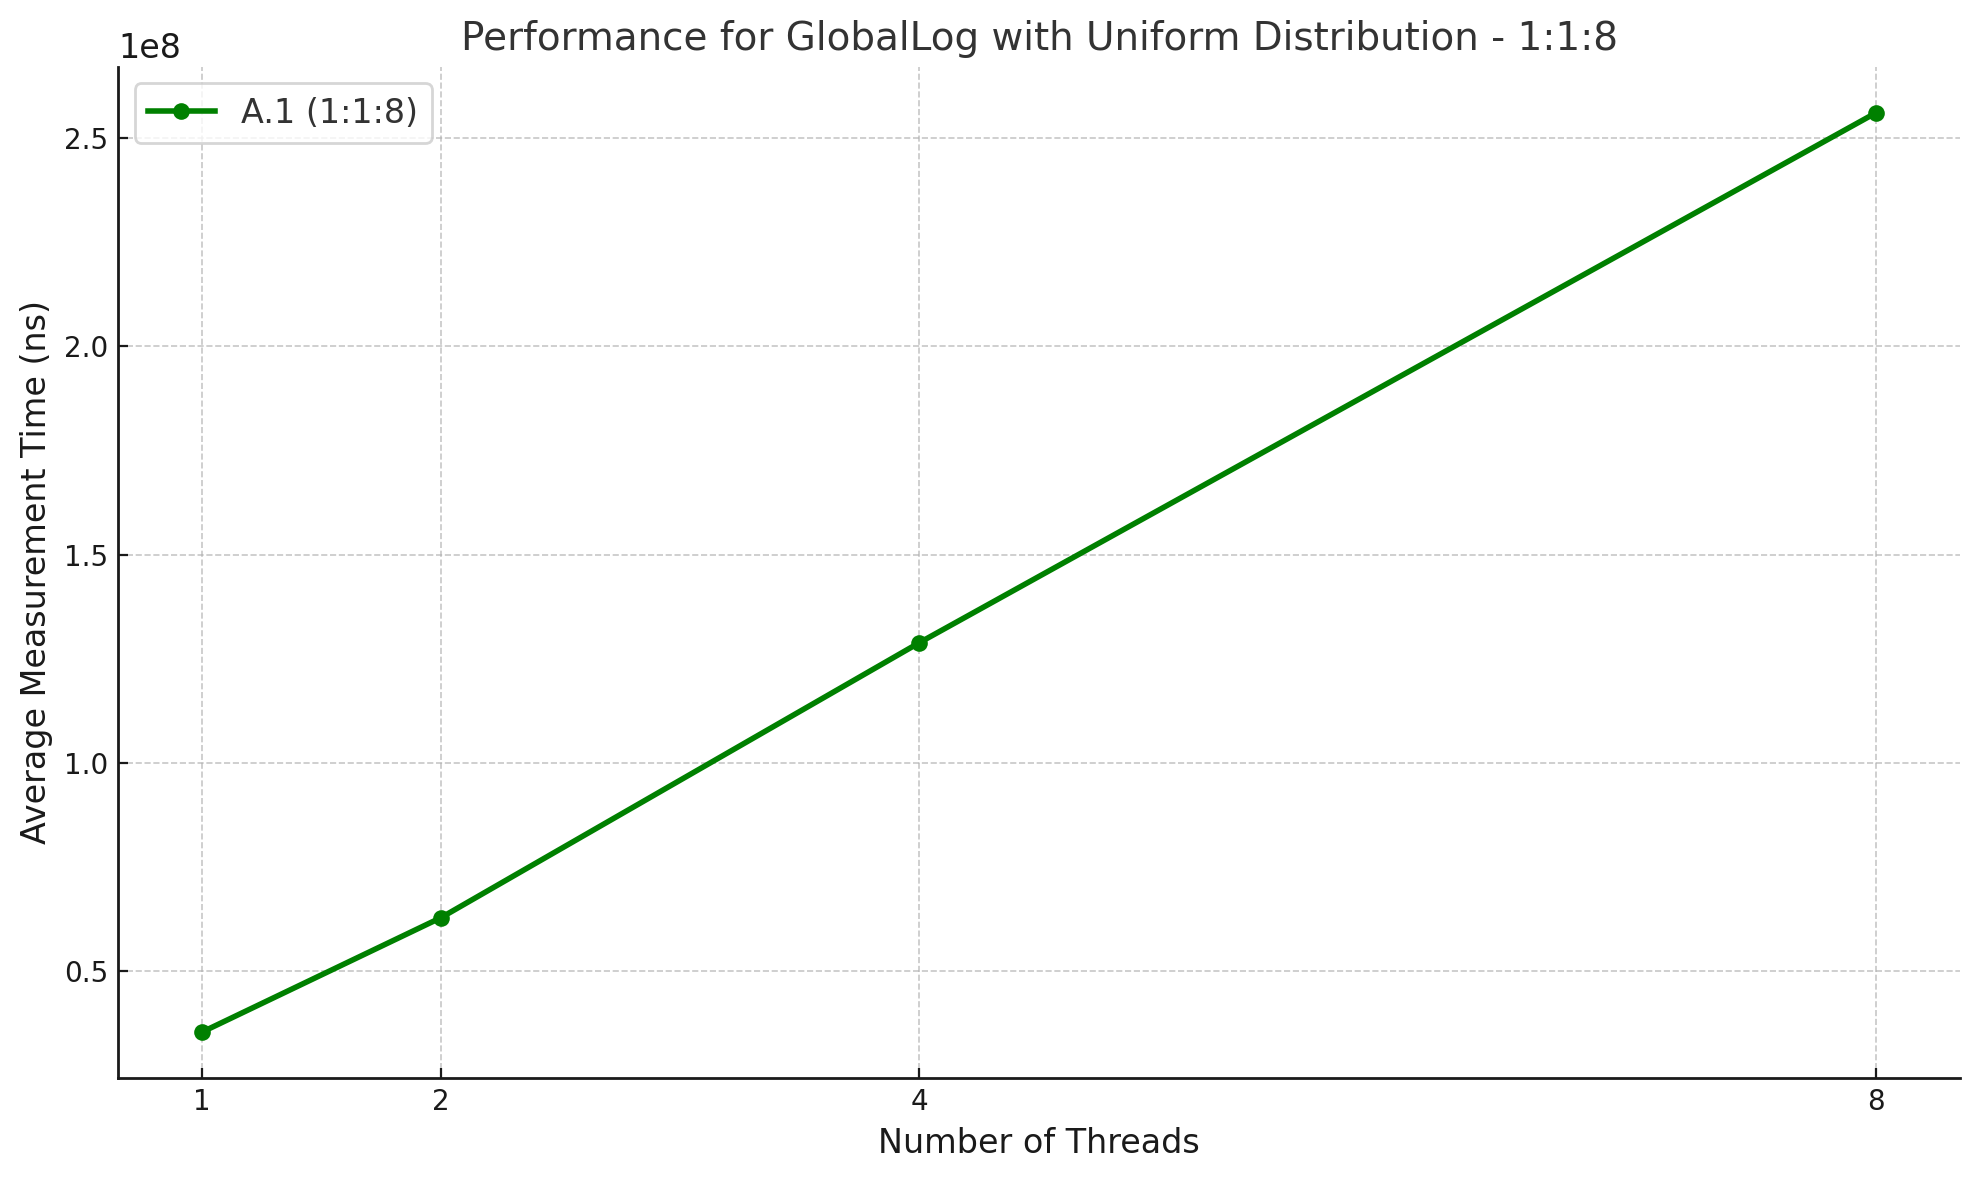
\includegraphics[width=\textwidth]{LaTex/images/Lab 3 2.5.2.1.png}
    \caption{Performance for GlobalLog}
    \label{fig:global-log-1-1-8}
\end{figure}

\begin{figure}[H]
    \centering
    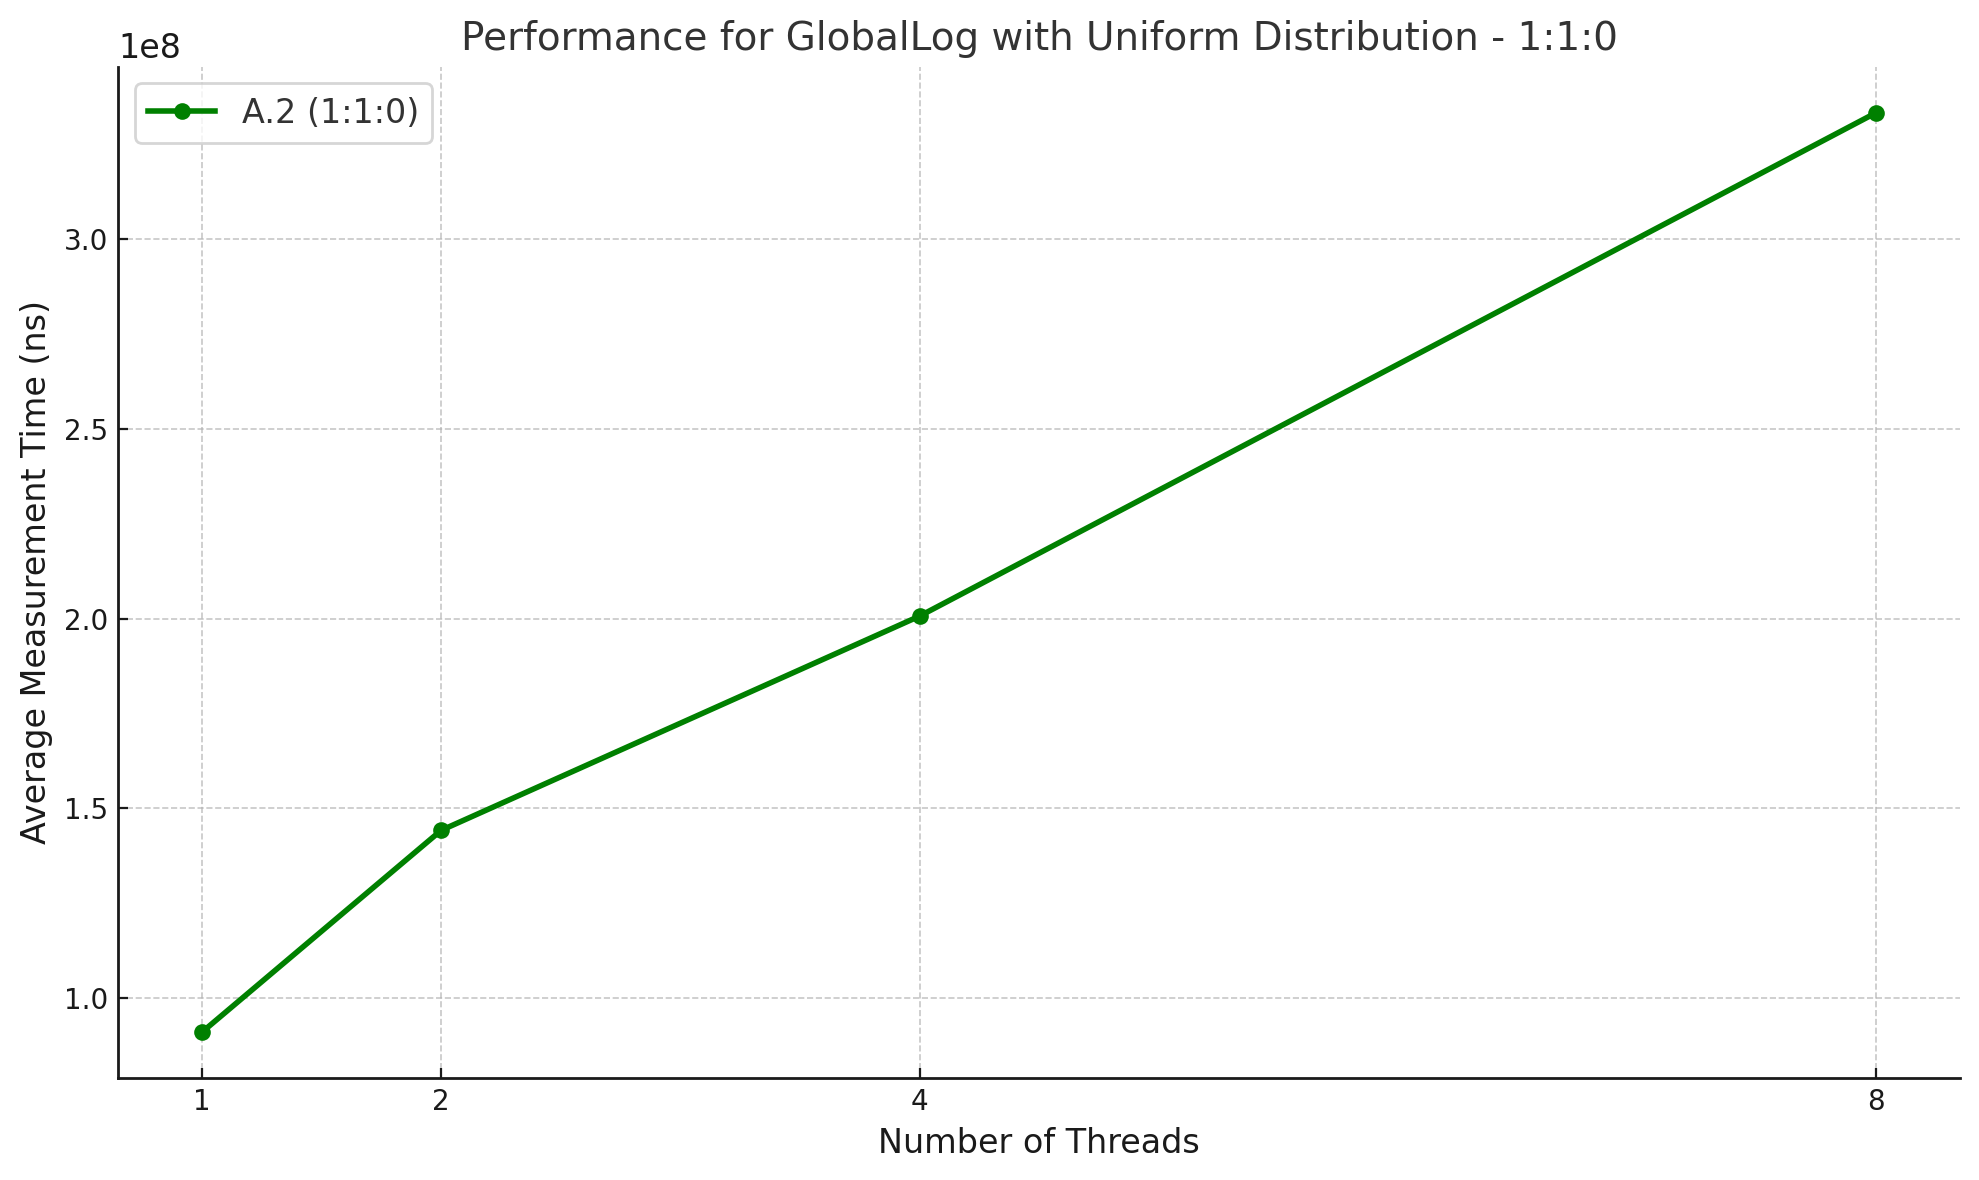
\includegraphics[width=\textwidth]{LaTex/images/Lab 3 2.5.2.2.png}
    \caption{Performance for GlobalLog - Extra Exercise}
    \label{fig:global-log-1-1-8}
\end{figure}

\begin{figure}[H]
    \centering
    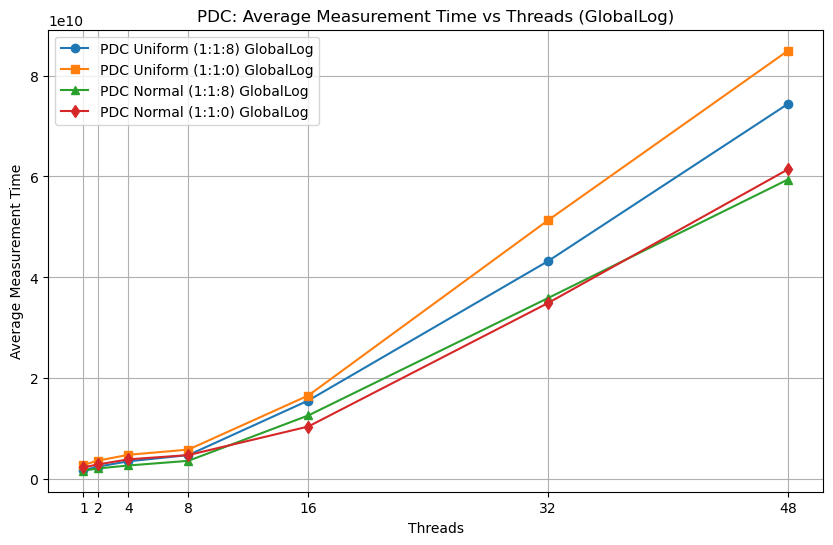
\includegraphics[width=\textwidth]{LaTex/images/Lab 3 2.5.2.3.png}
    \caption{Performance for GlobalLog - on Dardel}
    \label{fig:global-log-1-1-8}
\end{figure}

\begin{figure}[H]
    \centering
    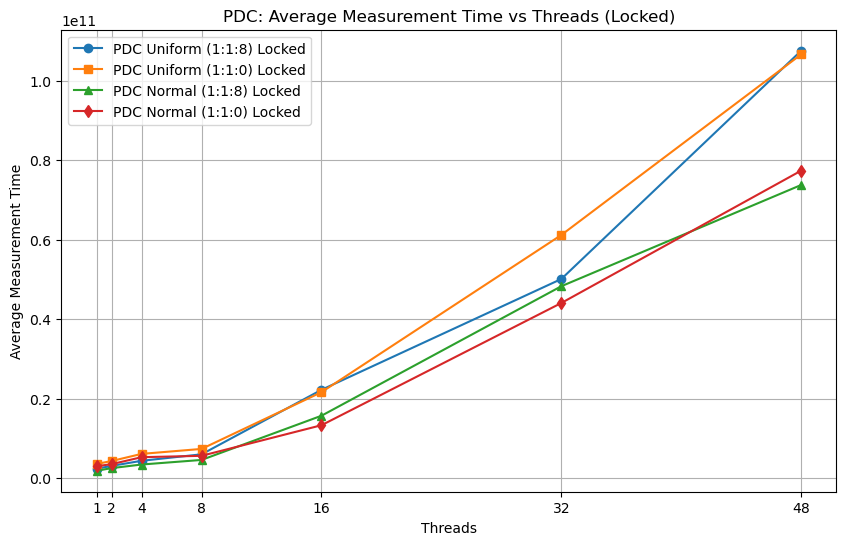
\includegraphics[width=\textwidth]{LaTex/images/Lab 3 2.5.2.4.png}
    \caption{Performance for GlobalLog - Extra Exercise - on Dardel}
    \label{fig:global-log-1-1-0}
\end{figure}

\subsubsection{Discussion}
The global log method demonstrated efficient performance scaling, particularly when using the lock-free queue mechanism. As the thread count increased, the method maintained near-linear scalability, indicating that the reduction in synchronization overhead was effective. The data from both local and Dardel experiments show that the average measurement time increased predictably with the number of threads, validating the method’s suitability for scenarios involving high-concurrency workloads.

Minor discrepancies observed at higher thread counts (particularly with 8 and above) are attributed to the concurrent interleaving of log entries, rather than inaccuracies in the time sampling mechanism itself. This suggests that while the global log approach may introduce some potential for minor inconsistencies under heavy contention, the overall accuracy remains consistently high.

The Dardel experiments, which included thread counts of up to 48, further confirm the scalability of this method in extreme scenarios. The observed trends validate that the global log method continues to perform well under larger thread counts, particularly with the mixtures B.1 (1:1:8) and B.2 (1:1:0). This underscores the method's capability to manage synchronization overhead effectively while maintaining reliable logging across highly concurrent operations, even as the workload scales dramatically.



\newpage
\printbibliography

\end{document}
